\documentclass[a4paper,11pt]{report}
\usepackage{kotex}
% 본문 내용 : 글자크기 11pt 정도, 줄간격 170 이상, 장평 100, 자간 0
\linespread{1.4} % 줄간격 170인듯?

% 각주 : 글자 크기 9~10pt

% 서체 : 명조체나 신명조체 류

% 용지 여백 : 위쪽 30, 아래쪽 15, 왼쪽 25, 오른쪽 25

\usepackage{graphicx}
\graphicspath{ {../images/} }

\begin{document}

% 논문 순서 1: 외표지
\begin{titlepage}
  \centering
  \begin{titlepage}
  \begin{center}
    {\fontsize{24}{24}\selectfont \textbf{희박한 확률 아래에서 인간의 합리성}}

    \vspace{0.5cm}

    {\fontsize{18}{18}\selectfont (The Access Control List based SecureOS)}

    \vspace{2cm}

    {\fontsize{18}{18}\selectfont 지도교수 : 하순회}

    \vspace{2cm}

    {\fontsize{20}{20}\selectfont 이 논문을 공학학사 학위 논문으로 제출함.}

    \vspace{2cm}

    {\fontsize{18}{18}\selectfont 2021년 6월 14일}

    \vspace{2cm}

    {\fontsize{20}{20}\selectfont 서울대학교 공과대학}

    \vspace{0.5cm}

    {\fontsize{20}{20}\selectfont 컴퓨터공학부}

    \vspace{0.5cm}

    {\fontsize{20}{20}\selectfont 홍 길 동}

    \vspace{2cm}

    {\fontsize{20}{20}\selectfont 2021년 8월}
  \end{center}
\end{titlepage}

\end{titlepage}

% 논문 순서 2: 속표지
\begin{titlepage}
  \centering
  \begin{titlepage}
  \begin{center}
    {\fontsize{24}{24}\selectfont \textbf{희박한 확률 아래에서 인간의 합리성}}

    \vspace{0.5cm}

    {\fontsize{18}{18}\selectfont (The Access Control List based SecureOS)}

    \vspace{2cm}

    {\fontsize{18}{18}\selectfont 지도교수 : 하순회}

    \vspace{2cm}

    {\fontsize{20}{20}\selectfont 이 논문을 공학학사 학위 논문으로 제출함.}

    \vspace{2cm}

    {\fontsize{18}{18}\selectfont 2021년 6월 14일}

    \vspace{2cm}

    {\fontsize{20}{20}\selectfont 서울대학교 공과대학}

    \vspace{0.5cm}

    {\fontsize{20}{20}\selectfont 컴퓨터공학부}

    \vspace{0.5cm}

    {\fontsize{20}{20}\selectfont 홍 길 동}

    \vspace{2cm}

    {\fontsize{20}{20}\selectfont 2021년 8월}
  \end{center}
\end{titlepage}

\end{titlepage}

% 논문 순서 3: 국문초록
\begin{abstract}
  \chapter*{국문초록}

\begin{center}
  \begin{minipage}{0.8\textwidth}
    본 연구는 St. Petersburg 역설을 해결하고 인간의 의사결정 과정을 분석하기 위해 시행 횟수-이익 확률 모델을 제안한다. 기존의 효용 함수나 외부적 제약에 의존한 접근과 달리, 본 연구는 반복 시행에서의 이익 확률에 초점을 맞춘다. 연구 결과, 이 역설은 무한한 기대값에서 비롯된 것이 아니라 희박한 보상 구조에서 이익 확률의 수렴 속도가 느리다는 데 기인함을 밝혔다. 참가 비용이 높아질수록 이익 확률의 수렴 속도는 더욱 감소하여, 높은 비용의 게임을 비합리적으로 판단하는 이유를 설명할 수 있었다. 본 모델은 낮은 확률과 높은 보상이 결합된 상황에서의 의사결정을 해석할 수 있는 새로운 틀을 제공하며, St. Petersburg 역설에 대한 통찰을 제시한다.
  \end{minipage}
\end{center}

\vspace{1em}
주요어 : 상트페테르부르크의 역설, 의사결정 이론, 기대효용이론

\end{abstract}

% 논문 순서 4: 목차
\tableofcontents

% 논문 순서 5: 본문
\chapter{서론}
연구의 배경 및 필요성: 연구 주제와 관련된 배경 지식 및 사회적/학문적 필요성을 설명합니다.

연구 목적: 연구에서 해결하려는 문제 또는 질문을 명확히 제시합니다.

연구 문제: 구체적인 연구 질문 또는 가설을 설정합니다.

연구 범위 및 한계: 연구의 범위를 설명하고, 논문에서 다루지 않는 부분(연구의 한계)도 명시합니다.

논문의 구조: 논문의 전개 흐름을 간략히 설명합니다.


\chapter{이론적 배경}
\section{기대값 기반의 결정 이론}

기대값 기반의 결정 이론은 어떤 선택의 기대값이 높을수록 그 선택을 하는 것이 합리적이라는 이론이다. (조사 필요)
어떤 선택의 기대값이 0 이상이면 그 선택을 하는 것이 합리적이라고 할 수 있다.

\section{St. Petersburg Paradox}

St. Petersburg Paradox는 기대값 계산 방식이 상식에 어긋나는 결과를 도출함을 보여주는 문제이다. St. Petersburg Game은 다음과 같은 규칙을 가진 게임이다. 참가자는 동전을 던져서 앞면이 나올 때까지 반복하고, 첫 번째로 앞면이 나오기까지 동전을 던진 횟수에 따라 상금을 받는다. 이때 동전을 던진 횟수를 X라고 하면 상금은 $2^X$원이다.

St. Petersburg Game에서 참가자가 얻을 수 있는 상금의 기대값은 다음과 같다.
\[
  \mathbf{E}[X] = \sum_{x=1}^{\infty} \frac{1}{2^x} \cdot 2^x = \sum_{x=1}^{\infty} 1 = \infty
\]

이론적으로 St. Petersburg Game의 기대값은 무한대이므로, 참가비가 아무리 높아도 그 금액이 유한하다면 이 게임에 참여하는 것이 합리적이어야 한다. 하지만 현실적으로는 사람들은 이 게임에 큰 돈을 지불하지 않으려고 한다.

\section{St. Petersburg Paradox에 대한 기존 해석}


\chapter{간단한 게임}
\section{간단한 게임}

St. Petersburg Game과 같은 의미를 지니지만 유한한 기대값을 가지는 게임을 통해 기대값 기반의 이론과 상식이 어긋나는 경우를 보여줄 수 있다. 참가자는 1/4 확률로 40원을 얻거나 3/4 확률로 0원을 얻는다. 이때 참가자가 얻는 상금의 기대값은 10원이다.

참가자는 참가 비용으로 상금의 기대값보다 낮은 금액을 지불한다면 게임에 참여하는 것이 합리적이다. 기대값 기반의 합리적인 이유를 다른 각도에서 바라보면, 참가자가 게임을 반복해서 참여했을 때 얻는 총 상금이 총 참가 비용보다 클 확률이 높기 때문이다. 즉 참가자가 본전을 찾을 확률이 높다면 게임에 참여하는 것이 합리적이다.

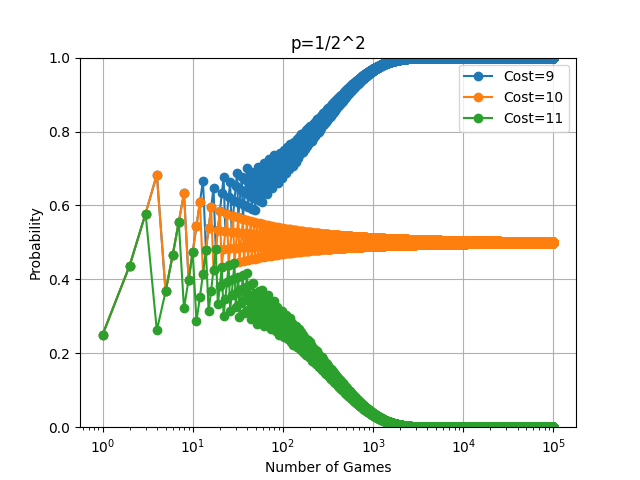
\includegraphics[width = \linewidth]{simple_game/E=2.png}

위 그림은 참가자가 게임을 반복해서 참여했을 때 본전을 찾을 확률을 나타낸 것이다. 참가자가 상금의 기대값보다 작은 금액을 지불한다면, 게임을 1000번 이상 참여했을 때 1에 가까운 확률로 돈을 잃지 않는다는 것을 알 수 있다. 참가자가 상금의 기대값과 같은 금액을 지불한다면, 본전을 찾을 확률이 50\%로 수렴하는 것을 볼 수 있다.


\section{희박한 확률 아래에서의 간단한 게임}

이제 간단한 게임을 변형하여 참가자가 $1/2^{10}$ 확률로 $10 \times 2^{10}$원을 얻거나 0원을 얻는 게임을 살펴보자. 이때 참가자가 얻는 상금의 기대값은 여전히 10원이다.

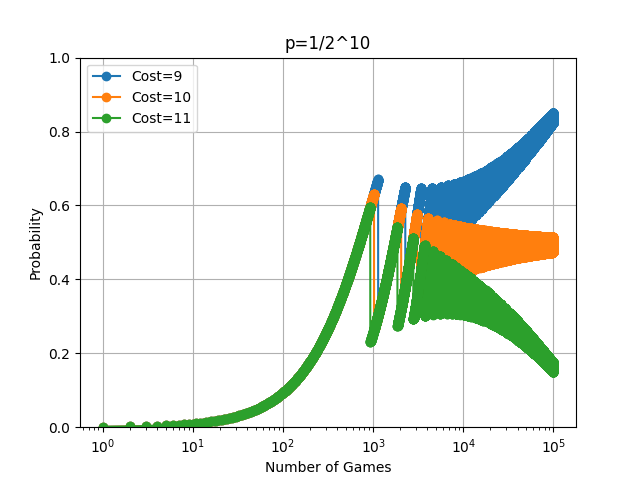
\includegraphics[width = \linewidth]{simple_game/E=10.png}

위 그림에서 참가자가 본전을 되찾을 확률은 상금의 기대값과 참가 비용에 따라서 여전히 1, 0.5, 0으로 수렴하려는 경향을 확인할 수 있다. 그러나 성공 확률이 1/4 인 게임보다 본전을 되찾을 확률이 수렴하는 속도가 느려진 것을 확인할 수 있다. 특히 게임을 100회 연속으로 참여하는 경우, 참가자가 1회도 성공하지 못하고 모든 참가 비용을 소모할 확률은 참가 비용과 상관 없는 것을 확인할 수 있다.


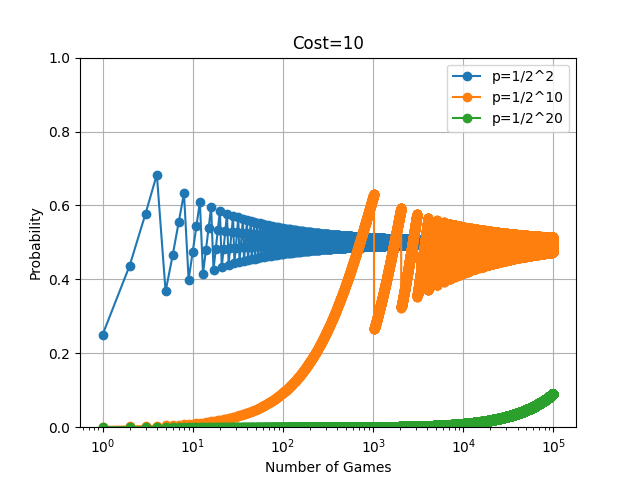
\includegraphics[width = \linewidth]{simple_game/cost=10.png}
위 그림은 상금의 기대값과 참가 비용이 같음에도 불구하고, 성공 확률이 희박해질 수록 참가자가 본전을 되찾을 확률이 0.5로 수렴하는 속도가 느려지는 것을 보인다.


\chapter{주장}
기대값 기반의 결정 이론은 선택의 기대값이 0 이상이라면 그 선택을 하는 것이 합리적이라고 판단한다. 본 논문에서 주장하려는 종류의 합리성은 인간은 본전을 되찾을 확률이 50\% 이상인 게임을 하는 것이 합리적이라고 판단한다는 것이다.

일반적인 확률 아래의 게임의 경우, 기대값 기반의 합리성과 본전을 찾을 확률을 고려한 합리성이 일치한다. 그러나 희박한 확률 아래의 게임에서는 기대값 기반의 합리성만 이용한다면 상식에 어긋나는 결과를 도출할 수 있다.

희박한 확률 아래의 게임에서는 게임의 기대값이 0 이상이더라도 efficient time 이내에 참가자가 본전을 찾을 확률이 낮다는 것이 그 이유이다.

희박한 확률 아래의 게임을 참가하는 인간은 기대값 뿐만 아니라 본전을 찾을 확률 또한 고려한다고 볼 수 있다.


\chapter{St. Petersburg Game}
참가자의 Cost에 따라 St petersburg 게임을 반복했을 때 본전을 찾을 확률이 얼마인지 그래프로 나타내려고 합니다.


\chapter{결론}

% 논문 순서 6: 참고문헌

% 논문 순서 7: (부록)

% 논문 순서 8: 영문초록
\begin{abstract}
  \chapter*{Abstract}

\vspace{1em}

{\centering
  \fontsize{22pt}{22pt}\selectfont An Interpretation of the St. Petersburg Paradox \\ using a Trial-Probability of Profit Model
  \par}

\vspace{2em}

\begin{center}
  \begin{minipage}{0.8\textwidth}
    {\raggedleft
      \fontsize{14pt}{14pt}\selectfont
      Gunwoo Kim\\
      Department of Computer Science and Engineering\\
      The Graduate School\\
      Seoul National University
      \par}
  \end{minipage}
\end{center}

\vspace{1em}

\begin{spacing}{1.2}
  \begin{center}
    \begin{minipage}{0.8\textwidth}
      This study proposes a trial-probability of profit model to address the St. Petersburg Paradox and analyze human decision-making processes. Unlike traditional approaches relying on utility functions or external constraints, this research focuses on the probability of profit over repeated trials. The findings reveal that the paradox stems not from infinite expected value but from the slow convergence in probability of profit under sparse reward structures. Experimental results demonstrate that higher participation costs further decelerate convergence in probability of profit, explaining why individuals deem high cost games irrational. The proposed model offers a novel framework for interpreting decision-making in scenarios involving low probability, high reward outcomes, providing insights into the St. Petersburg Paradox.
    \end{minipage}
  \end{center}
\end{spacing}

\vspace{1em}

keywords : St. Petersburg paradox, decision-making, expected utility

\end{abstract}

\end{document}
